%% LaTeX2e class for seminar theses
%% sections/content.tex
%% 
%% Karlsruhe Institute of Technology
%% Institute for Program Structures and Data Organization
%% Chair for Software Design and Quality (SDQ)
%%
%% Dr.-Ing. Erik Burger
%% burger@kit.edu
%%
%% Version 1.0, 2018-04-16

\section{Einf"uhrung}
Programmiersprachen haben unterschiedliche St"arken und Schw"achen. Das liegt daran, dass Sprachen meist f"ur ein bestimmtes Problem oder eine bestimmte Dom"ane an Problemen entwickelt werden. Schaut man sich Java und Prolog an, wird dies besonders deutlich. Java ist eine objekt-orientierte Programmiersprache mit dem Ziel, m"oglichst zug"anglich und gleichzeitig m"oglichst m"achtig zu sein. Durch den imperativen Programmierstil ist diese Sprache au"serdem f"ur viele Menschen gut verst"andlich und kann f"ur eine Vielzahl an Problemen eingesetzt werden. Prolog hingegen verfolgt einen ganz anderen Ansatz. Anstatt eine Sequenz an Befehlen zu programmieren, die angeben, \textit{wie} ein Problem gel"ost wird, definert man in Prolog lediglich \textit{was} das Problem ist und der Prolog-Interpreter l"ost es dann. Das ist vorallem dann von Vorteil, wenn man vorrangig logische Probleme l"osen will.

Um die Vorteile einer Sprache auch sprach"ubergreifend nutzen zu k"onnen, werden h"aufig Bibliotheken bereitgestellt, die als Schnittstelle zu anderen Sprachen dienen. Beispielsweise stellen einige Prolog-Interpreter Java-Bibliotheken bereit, die einen einfachen Zugang zu Prolog in Java-Code erm"oglichen. Allerdings haben diese Bibliotheken keine einheitliche API, was es erschwert, verschiedene Implementierungen derselben Sprach in einem Programm zu nutzen. Dabei ist eine Auswahl verschiedener Implentierungen genau das, was in manchen F"allen erforderlich sein kann. Gr"unde daf"ur k"onnen sich per Einsatzszenario "andernde Anforderungen sein, wie beispielsweise Lizenzbedingungen oder Performanceunterschiede. Um dennoch mehrere verschiedene Implemntierungen verwenden zu k"onnen, kapselt man die unterschiedlichen APIs in einem Adapter und stellt nach au"sen hin eine einheitliche API zur Verf"ugung. Abbildung \ref{fig:adpater} zeigt, wie ein solcher Adapter shematisch aussieht. Schnittstellen zu einer Zielsprache werden entweder als eine native Bibliothek zur Verf"ugung gestellt, oder die Zielsprach ist direkt in der Quellsprache implementiert. Der Adapter sellbst ist in der Quellsprache implementiert und kapselt die unterschiedlichen Schnittstellen-APIs. Dadurch kann das Hauptptogramm einheitlich auf die verschiedenen Implementierungen der Zielsprache zugreifen.

\begin{figure}[h]
\centering
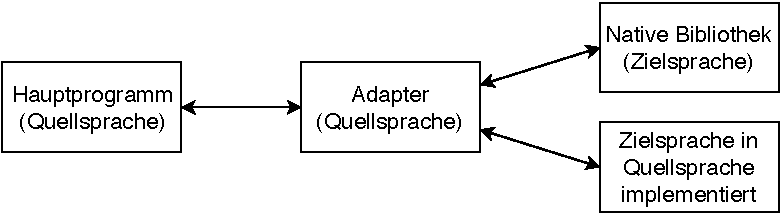
\includegraphics[width=0.8\textwidth]{adapter.pdf}
\caption{Ein Adapter ist in der Quellsprache implementiert und greift entweder auf eine native Bibliothek oder auf eine Quellsprach-Implementierung der Zielsprache zu.}
\label{fig:adpater}
\end{figure}

\subsection{Projektrahmen}
\label{projektrahmen}
Dieses Praktikum findet im Rahmen des Projektes Trust 4.0\cite{trust40} statt. Trust 4.0 hat es sich als Ziel gesetzt, Datenschutz in einem Softwaresystem garantieren zu k"onnen. Dazu wird mittels eines Plugins in Eclipse ein Architekturmodell des zu pr"ufenden Softwaresystems erstellt und um Datenflussannotationen erg"anzt. Diese Annotation beschreiben, welchen Weg personenbezogne Daten "uber verschiedene Software-Module hinweg nehmen und aufgrunddessen kann man analysieren, ob es an einer Stelle zu Datenlecks kommen kann. Das Eclipse-Plugin selbst ist in Java implementiert, jedoch hat man sich bei der Datenflussanalyse f"ur Prolog entschieden.  Wie bereist weiter oben erl"autert, ist Prolog speziell f"ur rein logischen Probleme entwickelt worden, weshalb es sich f"ur die Analyse besser eignet als Java. Um es in Zukunft dem Nutzer zu erm"oglichen, von dem Eclipse-Plugin aus die Analyse auf einem frei gew"ahlten Prolog-Interpreter auszuf"uhren, ist es das Ziel dieses Praktikums, einen Prolog-Adapter f"ur Java zu entwickeln.
